\documentclass[a4paper]{article}
\usepackage[english]{babel}
\usepackage[utf8]{inputenc}
\usepackage{amsmath}
\usepackage{graphicx}
\usepackage{natbib}
\usepackage{float}
\usepackage[margin=1.2in]{geometry}
\usepackage{caption}
\usepackage{subcaption}
\usepackage{url}
\usepackage{bm}
\usepackage{wasysym}
\usepackage{pdflscape}
\usepackage{tabularx}
\usepackage{hhline}
\usepackage{geometry}
\usepackage{longtable}
\usepackage{amsmath,bm}
\usepackage{array}
\usepackage{mathtools}
\usepackage{setspace}
\usepackage{siunitx}
%\usepackage{hyperref}
\onehalfspacing

\mathchardef\mhyphen="2D

\newcommand{\pder}[2][]{\frac{\partial#1}{\partial#2}}
\newcommand{\pdder}[2][]{\frac{\partial^2#1}{\partial#2 ^2}}
\newcolumntype{P}[1]{>{\centering\arraybackslash}p{#1}}

\graphicspath{{./../plots/}}

%----------------------------------------------------------------------------------------

\title{Time Series\\ Practical 1}

\author{Rory Hetherington (200471193)}

\date{22 Mar 2017}

\begin{document}


\maketitle

%----------------------------------------------------------------------------------------

\begin{abstract}
	\centering
	You should start your report with a short (1 paragraph)	summary of your findings, written in a style suitable for a non-statistician.
\end{abstract}

%----------------------------------------------------------------------------------------

\section*{Question 1}
The pond data, which contains the monthly water levels in a small pond in rural Hampshire, is loaded into \textsf{R}. Recordings are taken at the start of every month, from January 1966 to December 2015. Without performing any processing of raw data, the following are noted

\begin{itemize}
	\item The measuring appears to have a maximum cutoff at \SI{6}{m}. Anything above this gets set to \SI{6}{m}. 
	\item There are seasonality effects with a period of 12 months. 
	\item A seasonal effect with a period greater than 12 months is present. This is approximated at 8.5 years.
	\item One large dip in the data, where the pond level reaches a record low, is seen around 2005. This 
\end{itemize}

The data is plotted (Figure \ref{fig:plot_data}) and summary statistics are computed (Table \ref{tab:summary_stats}).

\begin{figure} [H]
	\centering
	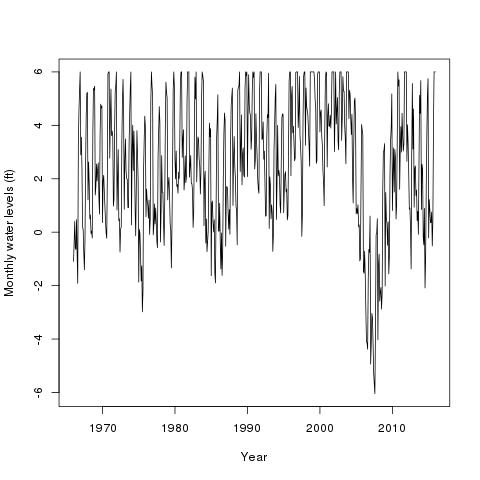
\includegraphics[width=0.6\textwidth]{plot_data}
	\caption{Monthly water levels in a pond.}
	\label{fig:plot_data}
\end{figure}

By plotting the ACF of the pond data time series, we see a periodic seasonality is present in the data (Figure \ref{fig:plot_acf}).

\begin{figure} [H]
	\centering
	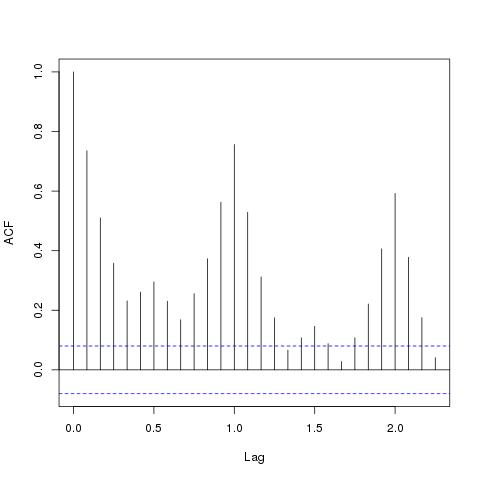
\includegraphics[width=0.6\textwidth]{plot_acf}
	\caption{ACF of data.}
	\label{fig:plot_acf}
\end{figure}


\begin{longtable}{ p{.1\textwidth} P{.1\textwidth}  P{.1\textwidth}    P{.1\textwidth}    P{.1\textwidth}   P{.1\textwidth} }
	\hline \hline  \vspace{0.2cm}
	\textbf{Min.}  & \textbf{1st Qu.}  &  \textbf{Median}  &  \textbf{Mean}   &  \textbf{3rd Qu.} &   \textbf{Max.}\\ 
	\hline 
	-6.0460 &   0.7135   &  2.6400  &   2.5180    &   4.4540  &    6.0000    \\	
	\hline \hline
	\caption{Summary statistics for monthly water levels in a pond.}
	\label{tab:summary_stats}
\end{longtable}

Seasonality (annual) was removed and residuals were denoted by $Y$ (see Figure \ref{fig:plot_data_residuals}). It can be seen from the plot that there exists a seasonality trend of approximately 8.5 years.

\begin{figure} [H]
	\centering
	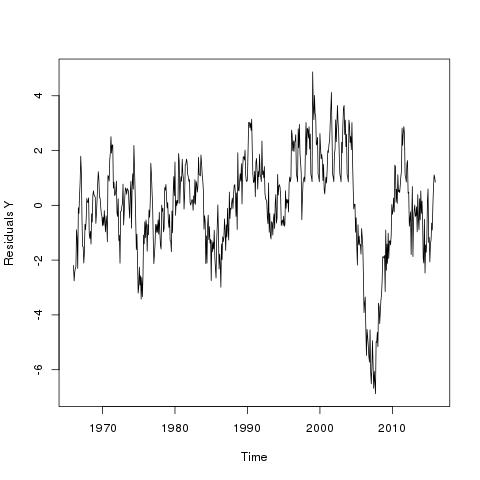
\includegraphics[width=0.6\textwidth]{plot_data_residuals}
	\caption{Residuals $Y$.}
	\label{fig:plot_data_residuals}
\end{figure}

The ACF of the residuals $Y$ is plotted, it is evident that there exists a trend in the data (Figure \ref{fig:plot_residual_acf}).

\begin{figure} [H]
	\centering
	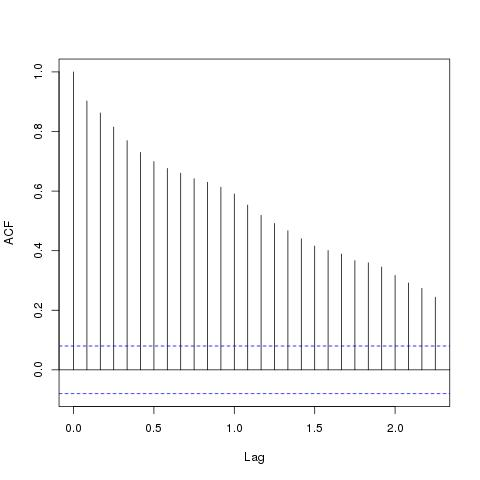
\includegraphics[width=0.6\textwidth]{plot_residual_acf}
	\caption{ACF of residuals $Y$.}
	\label{fig:plot_residual_acf}
\end{figure}






\end{document}